\subsection{Considering I/O Configurations}
\makesubcontentsslidessec

\begin{frame}{I/O Configurations}
\vspace{-1em}
  \begin{minipage}{0.32\textwidth}
    \begin{block}{Best!}
      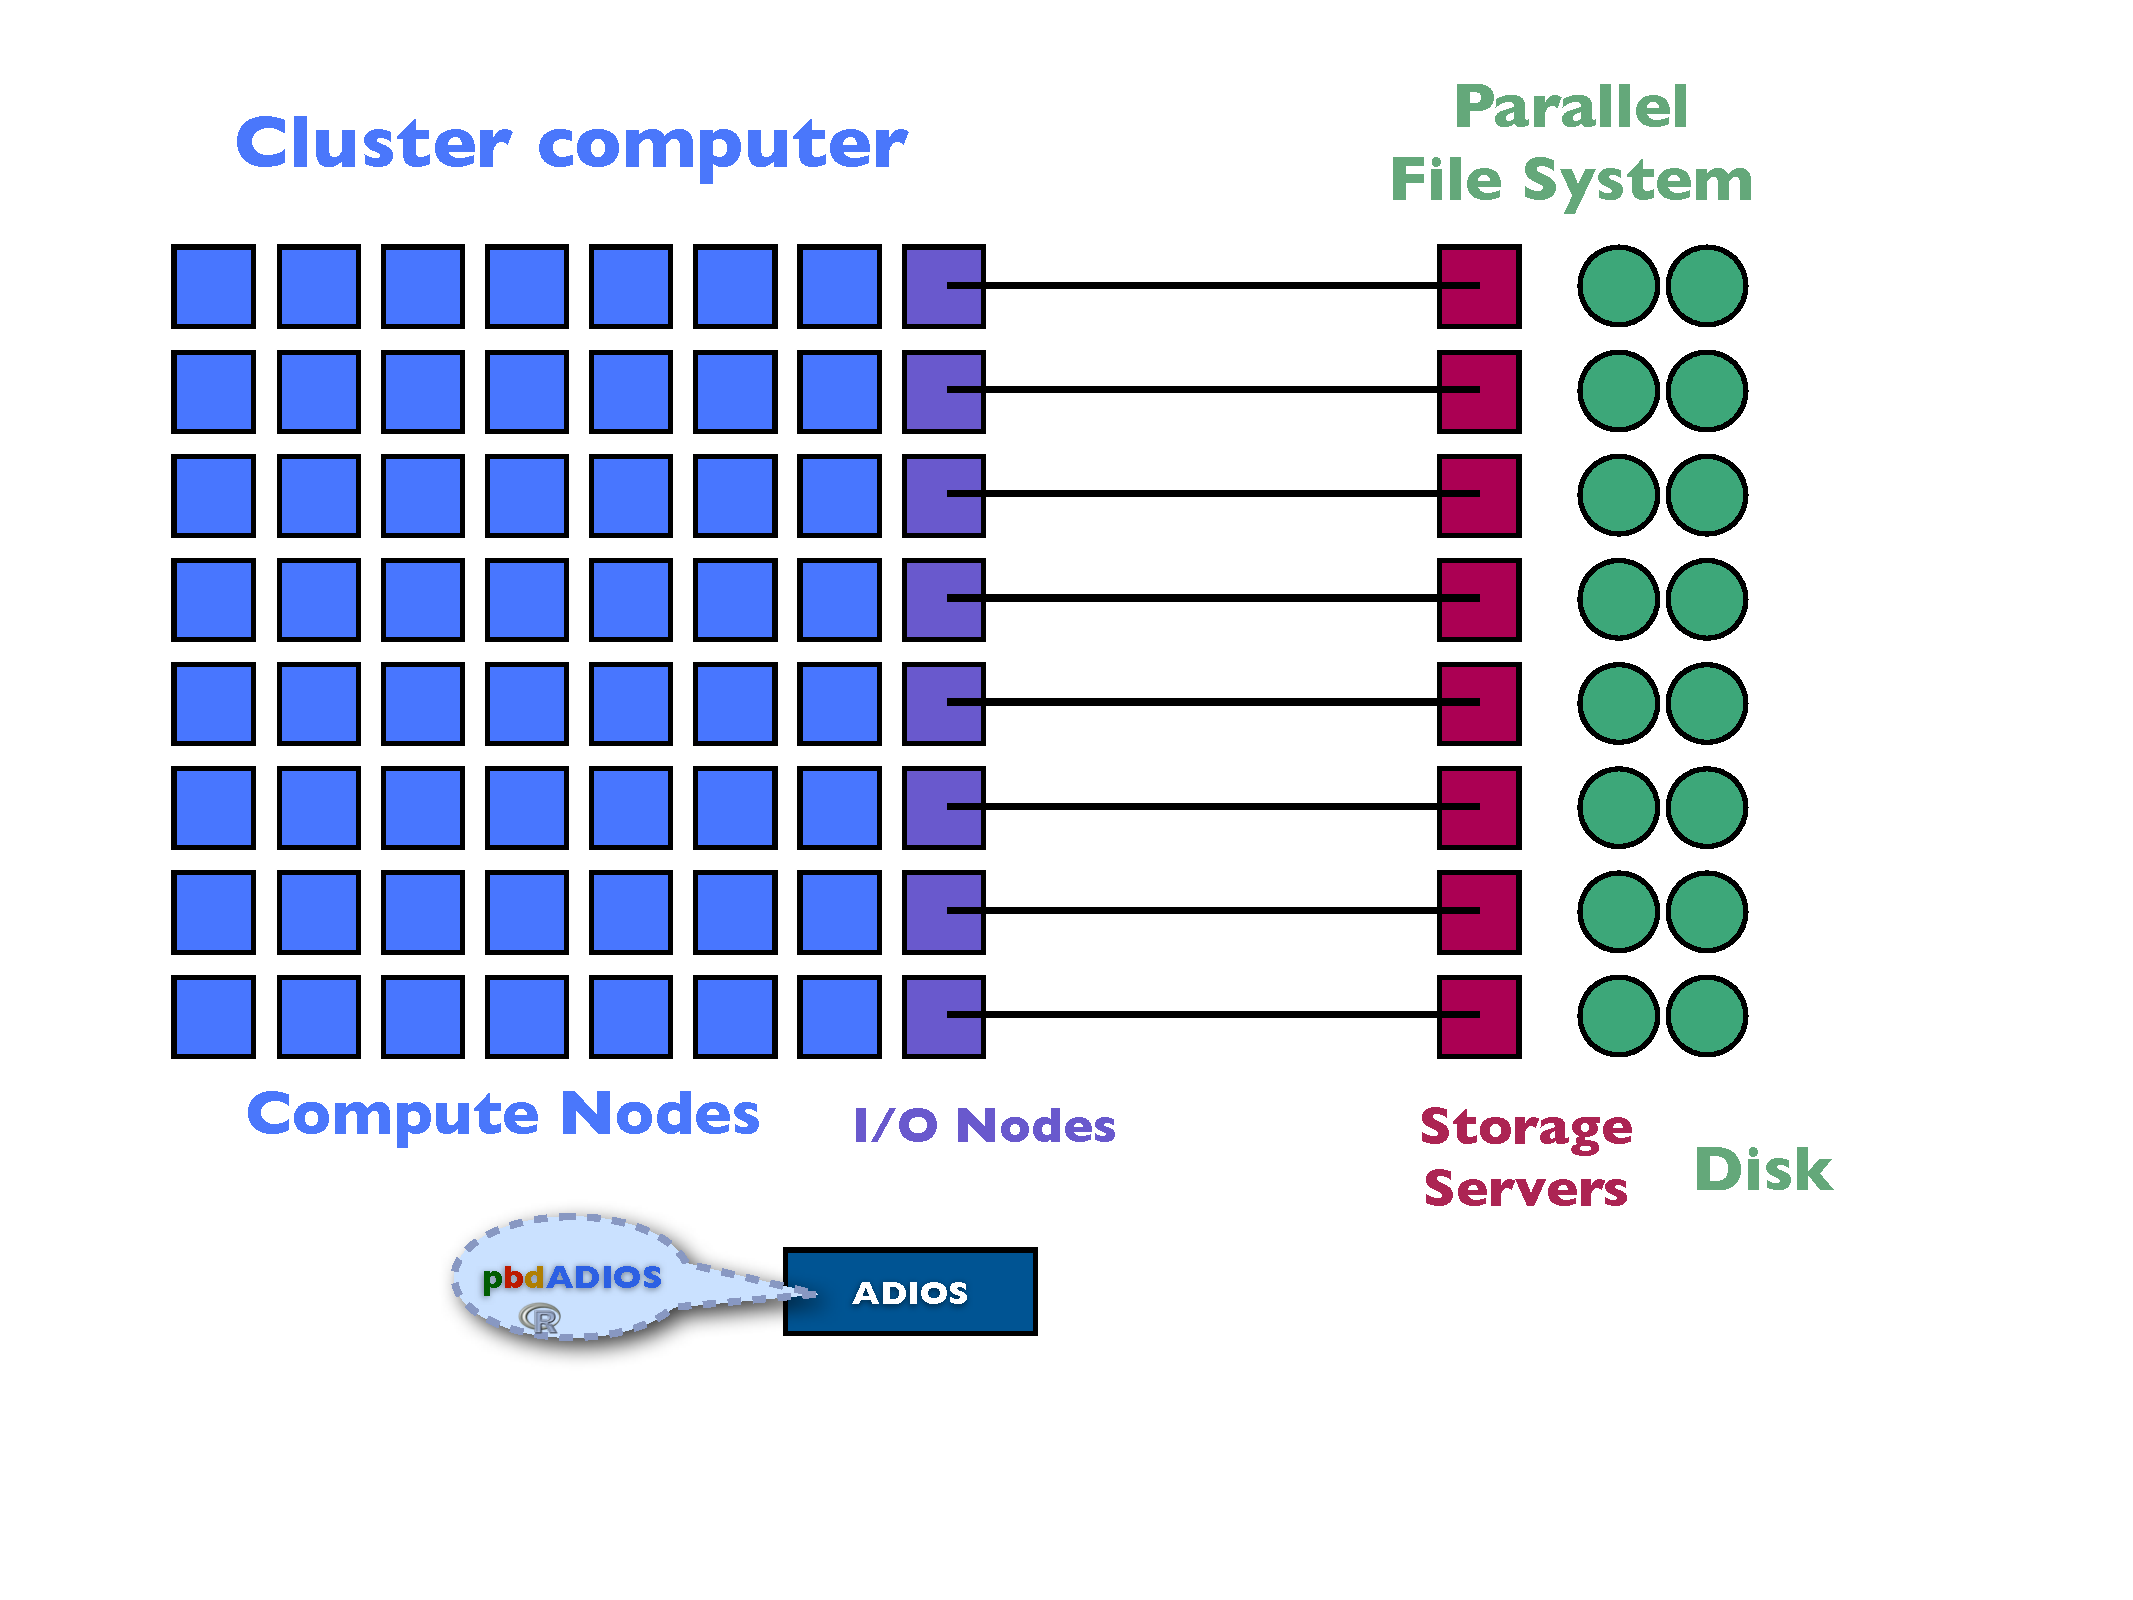
\includegraphics[trim=0 120 30 40,clip,width=1\textwidth]{../common/pics/hardware/ParallelHardware20.pdf}
    \end{block}
  \end{minipage}\hspace{1ex}
  \begin{minipage}{0.32\textwidth}
    \begin{block}{Good.}
      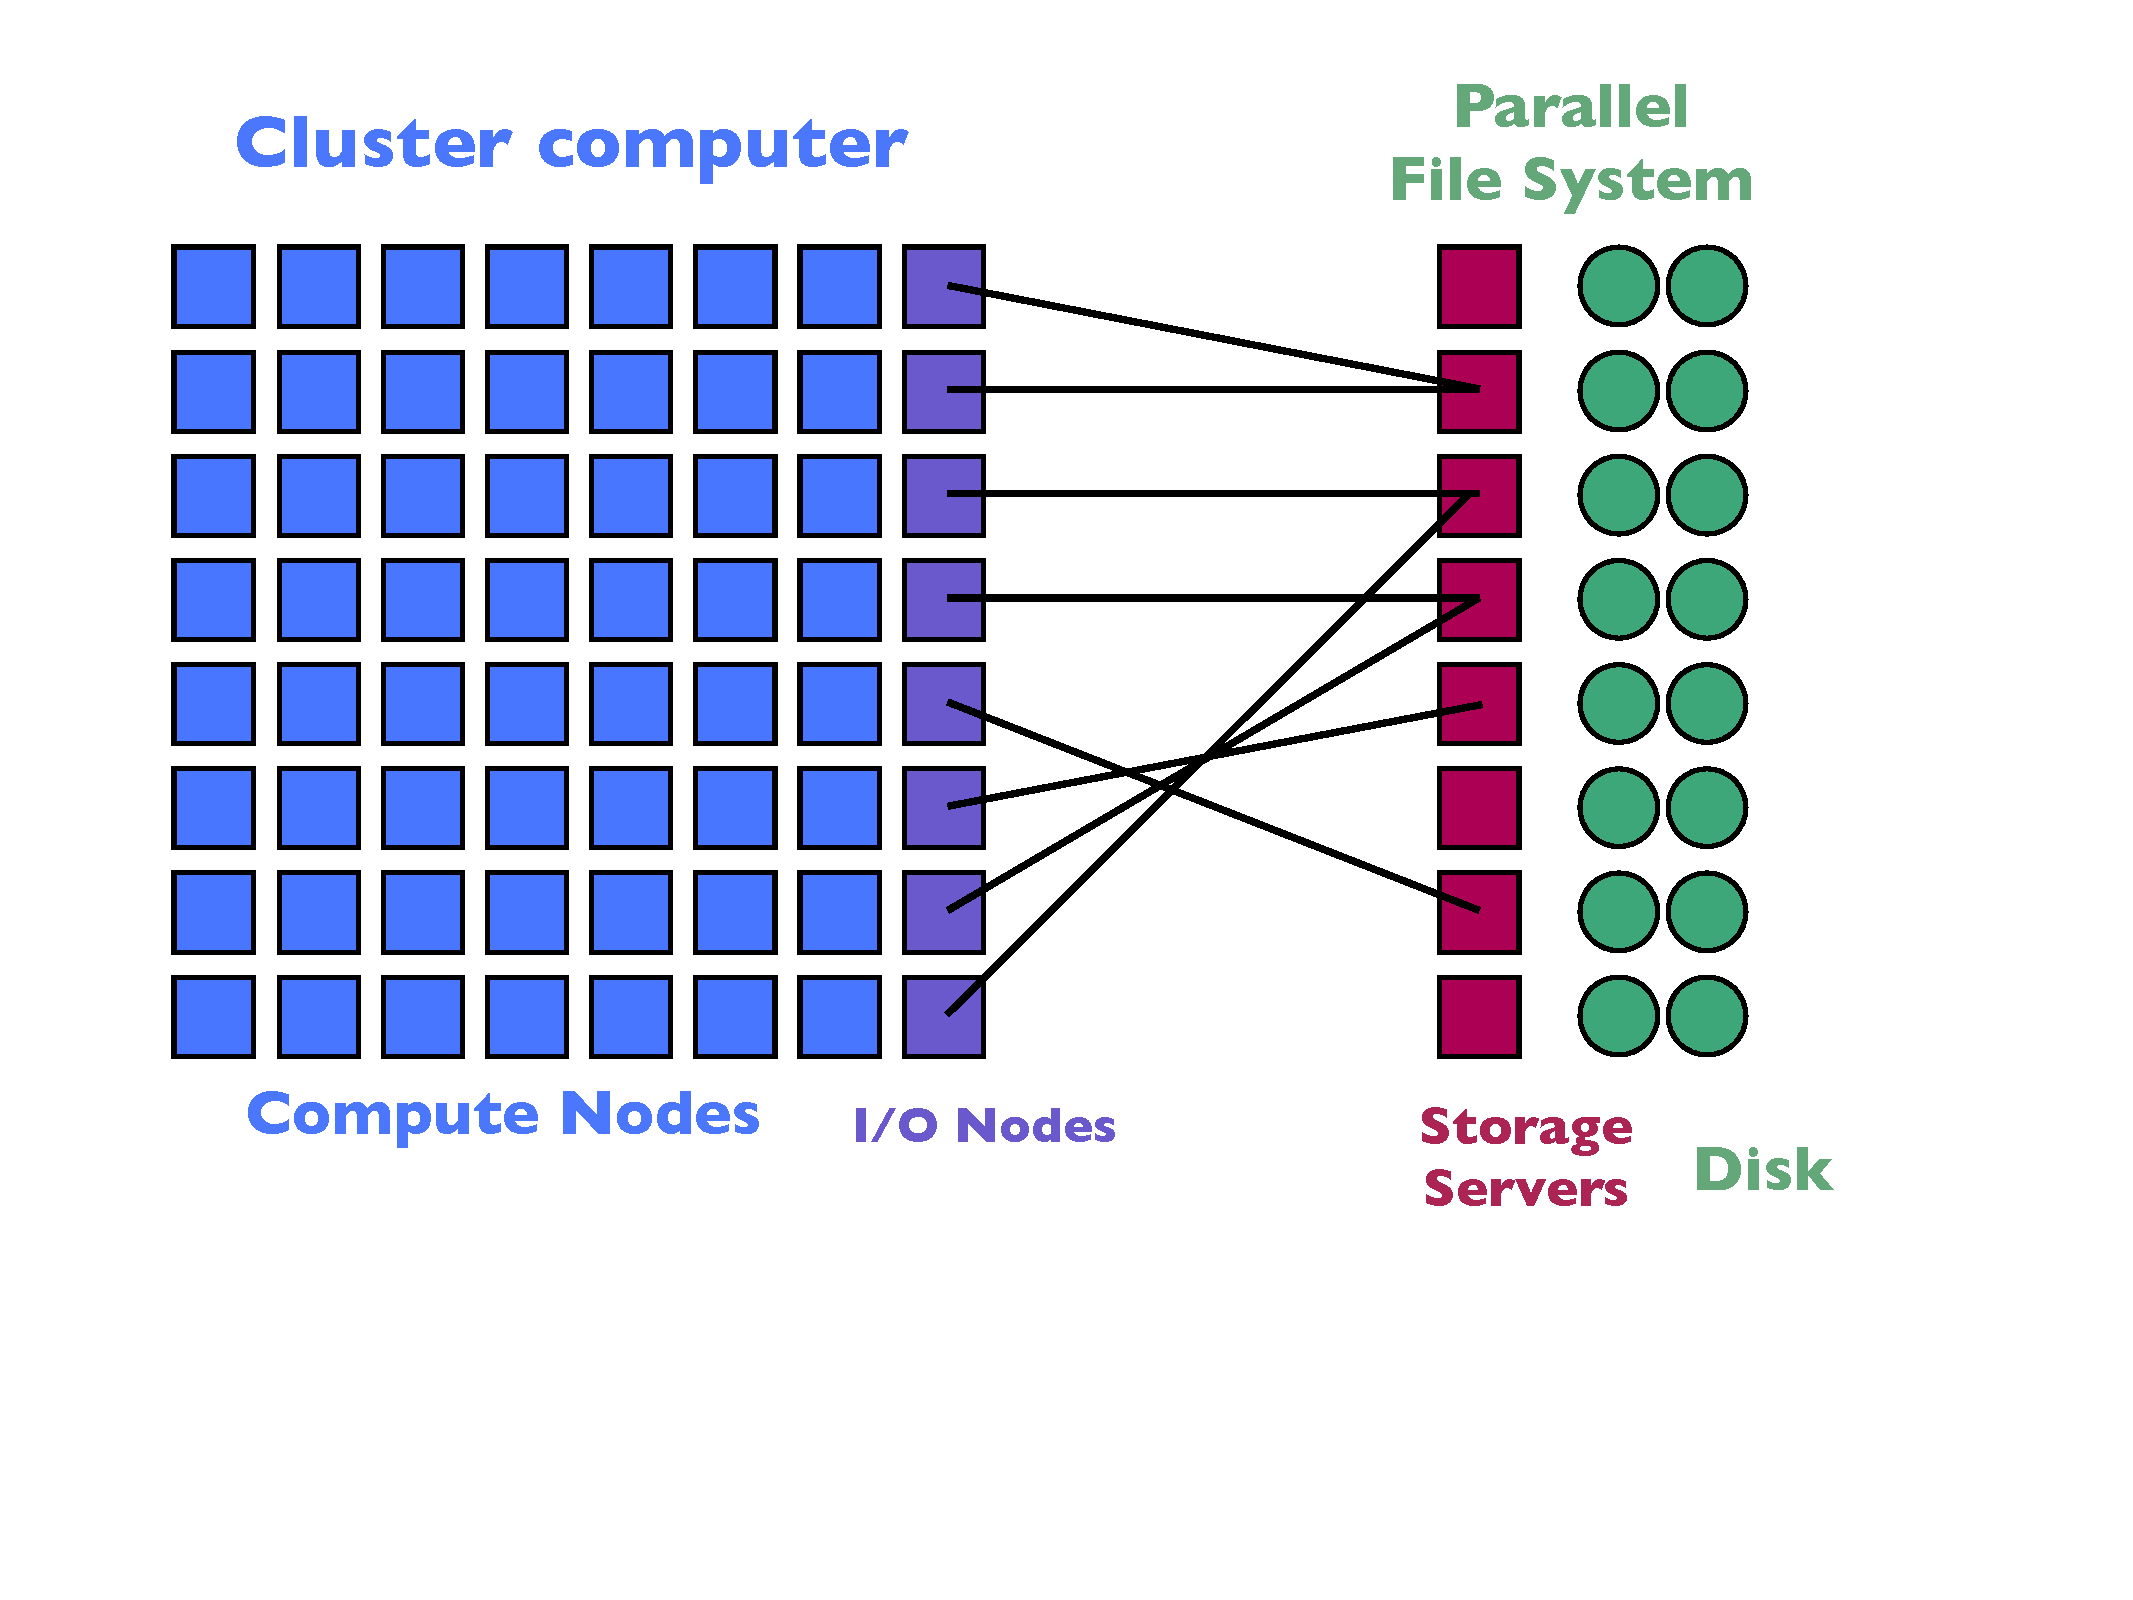
\includegraphics[trim=0 120 30 40,clip,width=1\textwidth]{../common/pics/hardware/ParallelHardware19.pdf}
    \end{block}
  \end{minipage}\hspace{1ex}
  \begin{minipage}{0.32\textwidth}
    \begin{block}{If you have to.}
      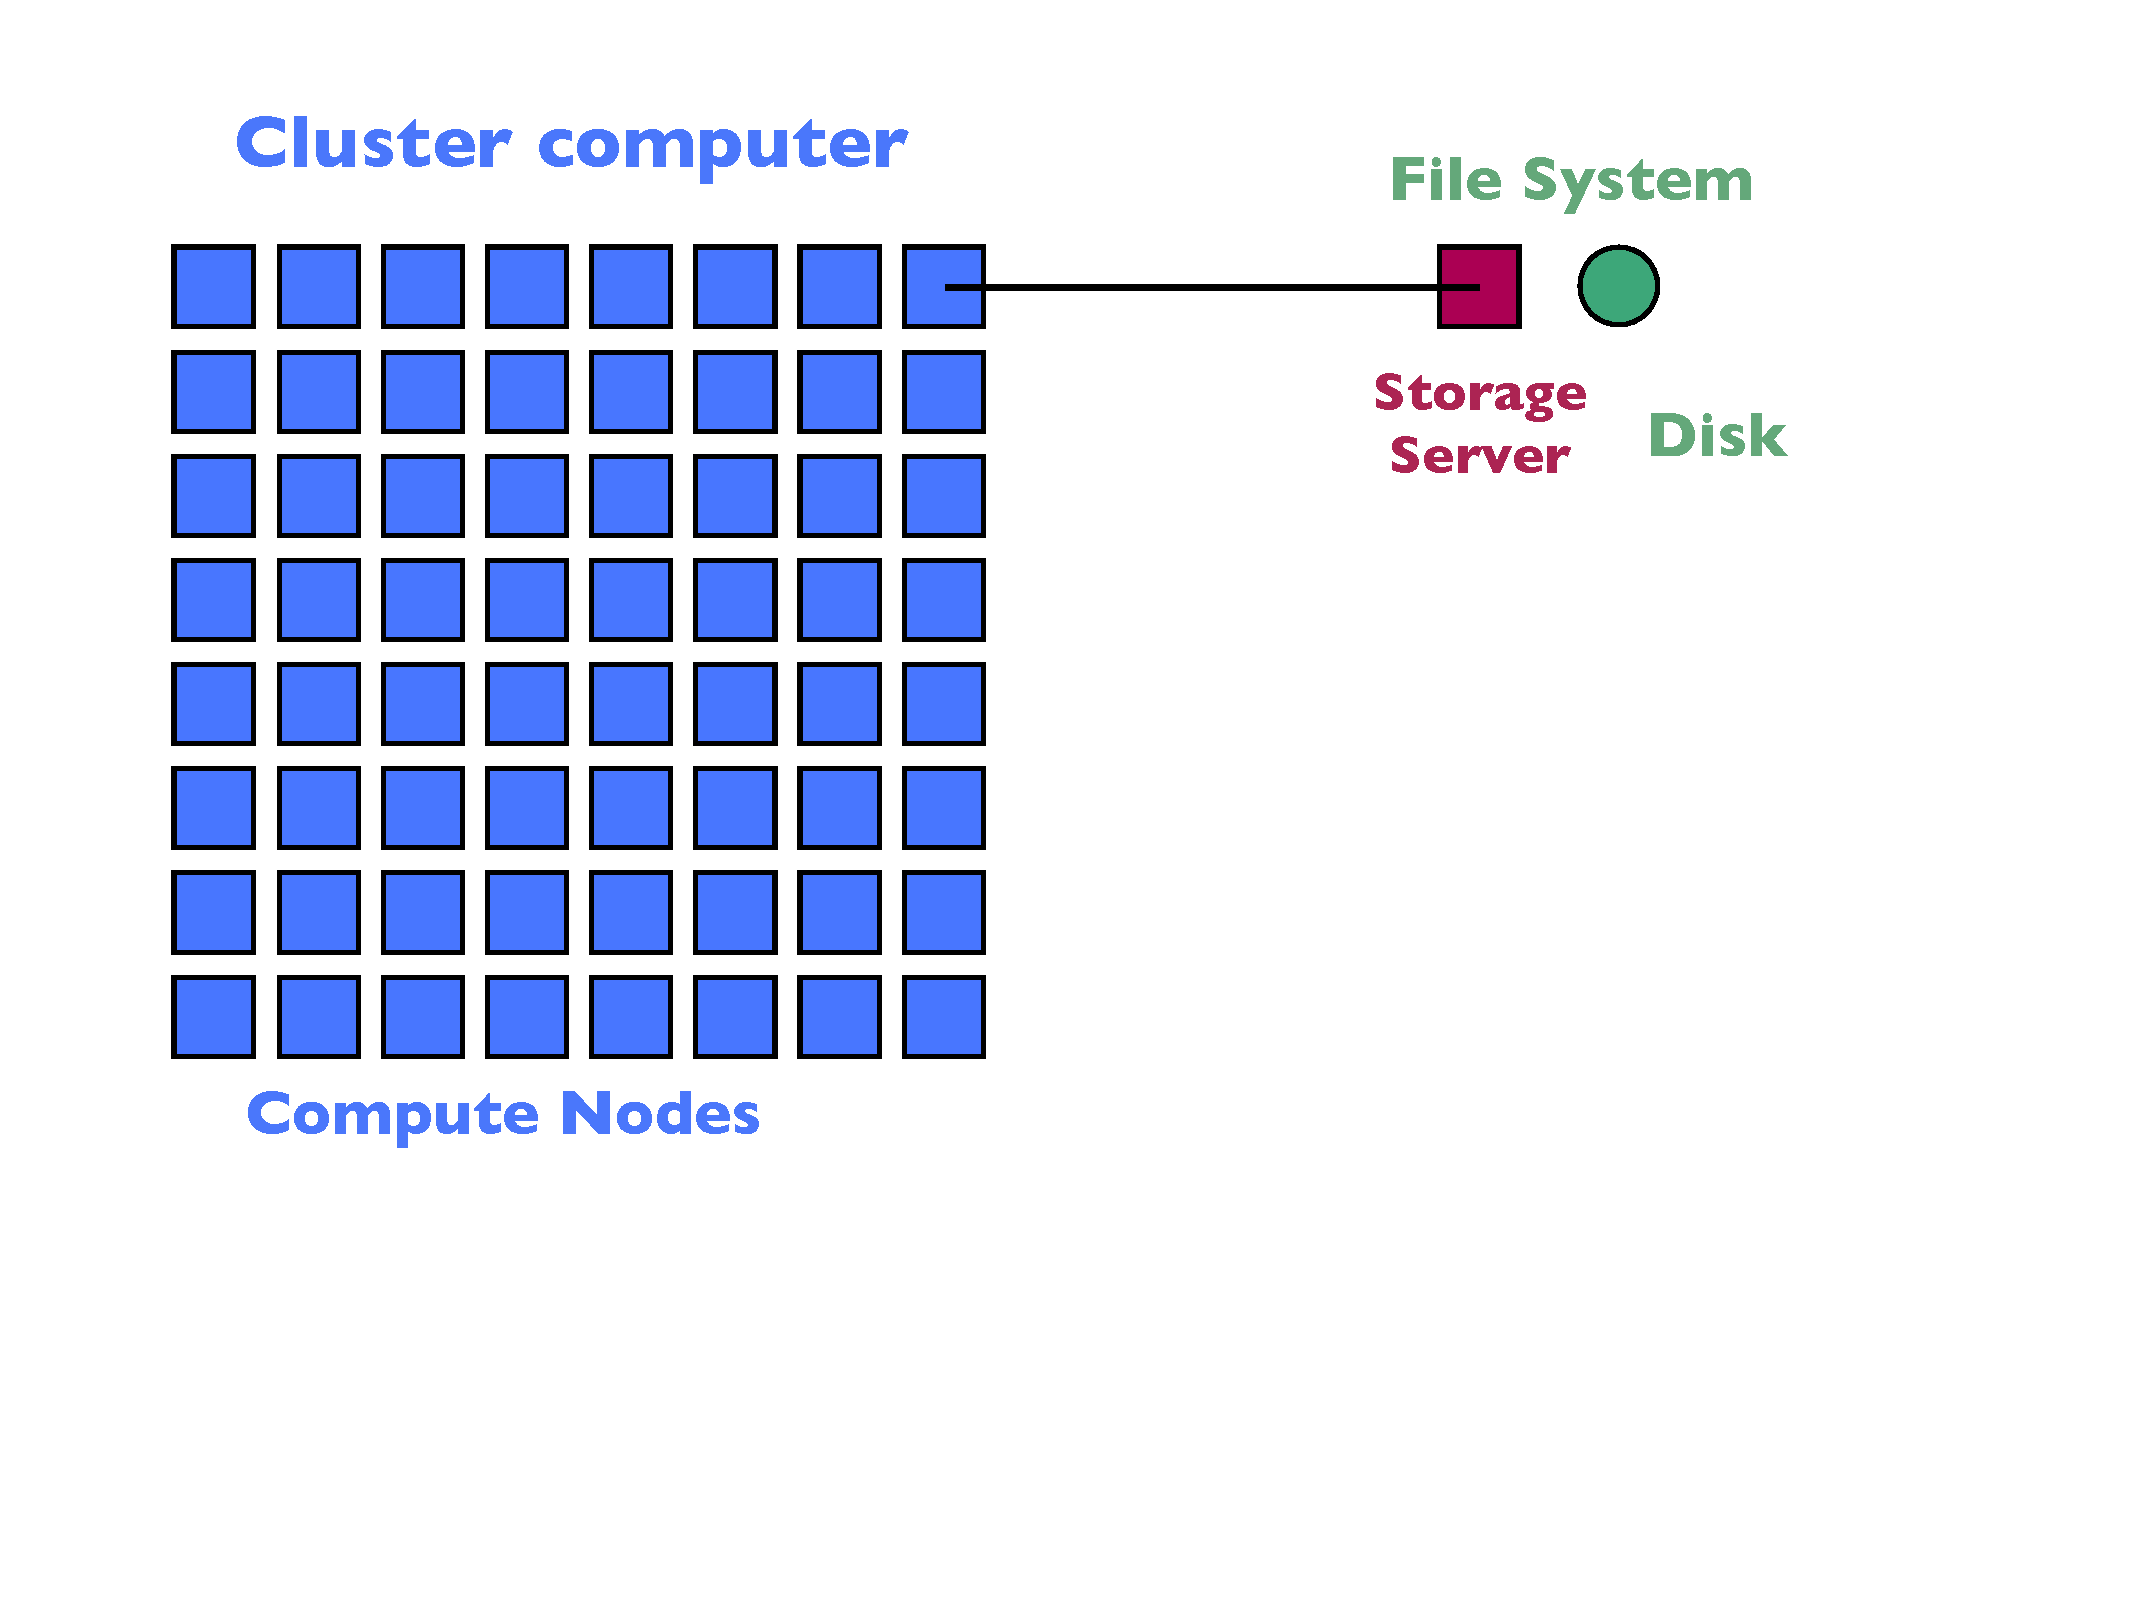
\includegraphics[trim=0 120 30 40,clip,width=1\textwidth]{../common/pics/hardware/ParallelHardware15.pdf}
    \end{block}
  \end{minipage}
  \begin{minipage}{0.32\textwidth}
    \begin{block}{Can work.}
      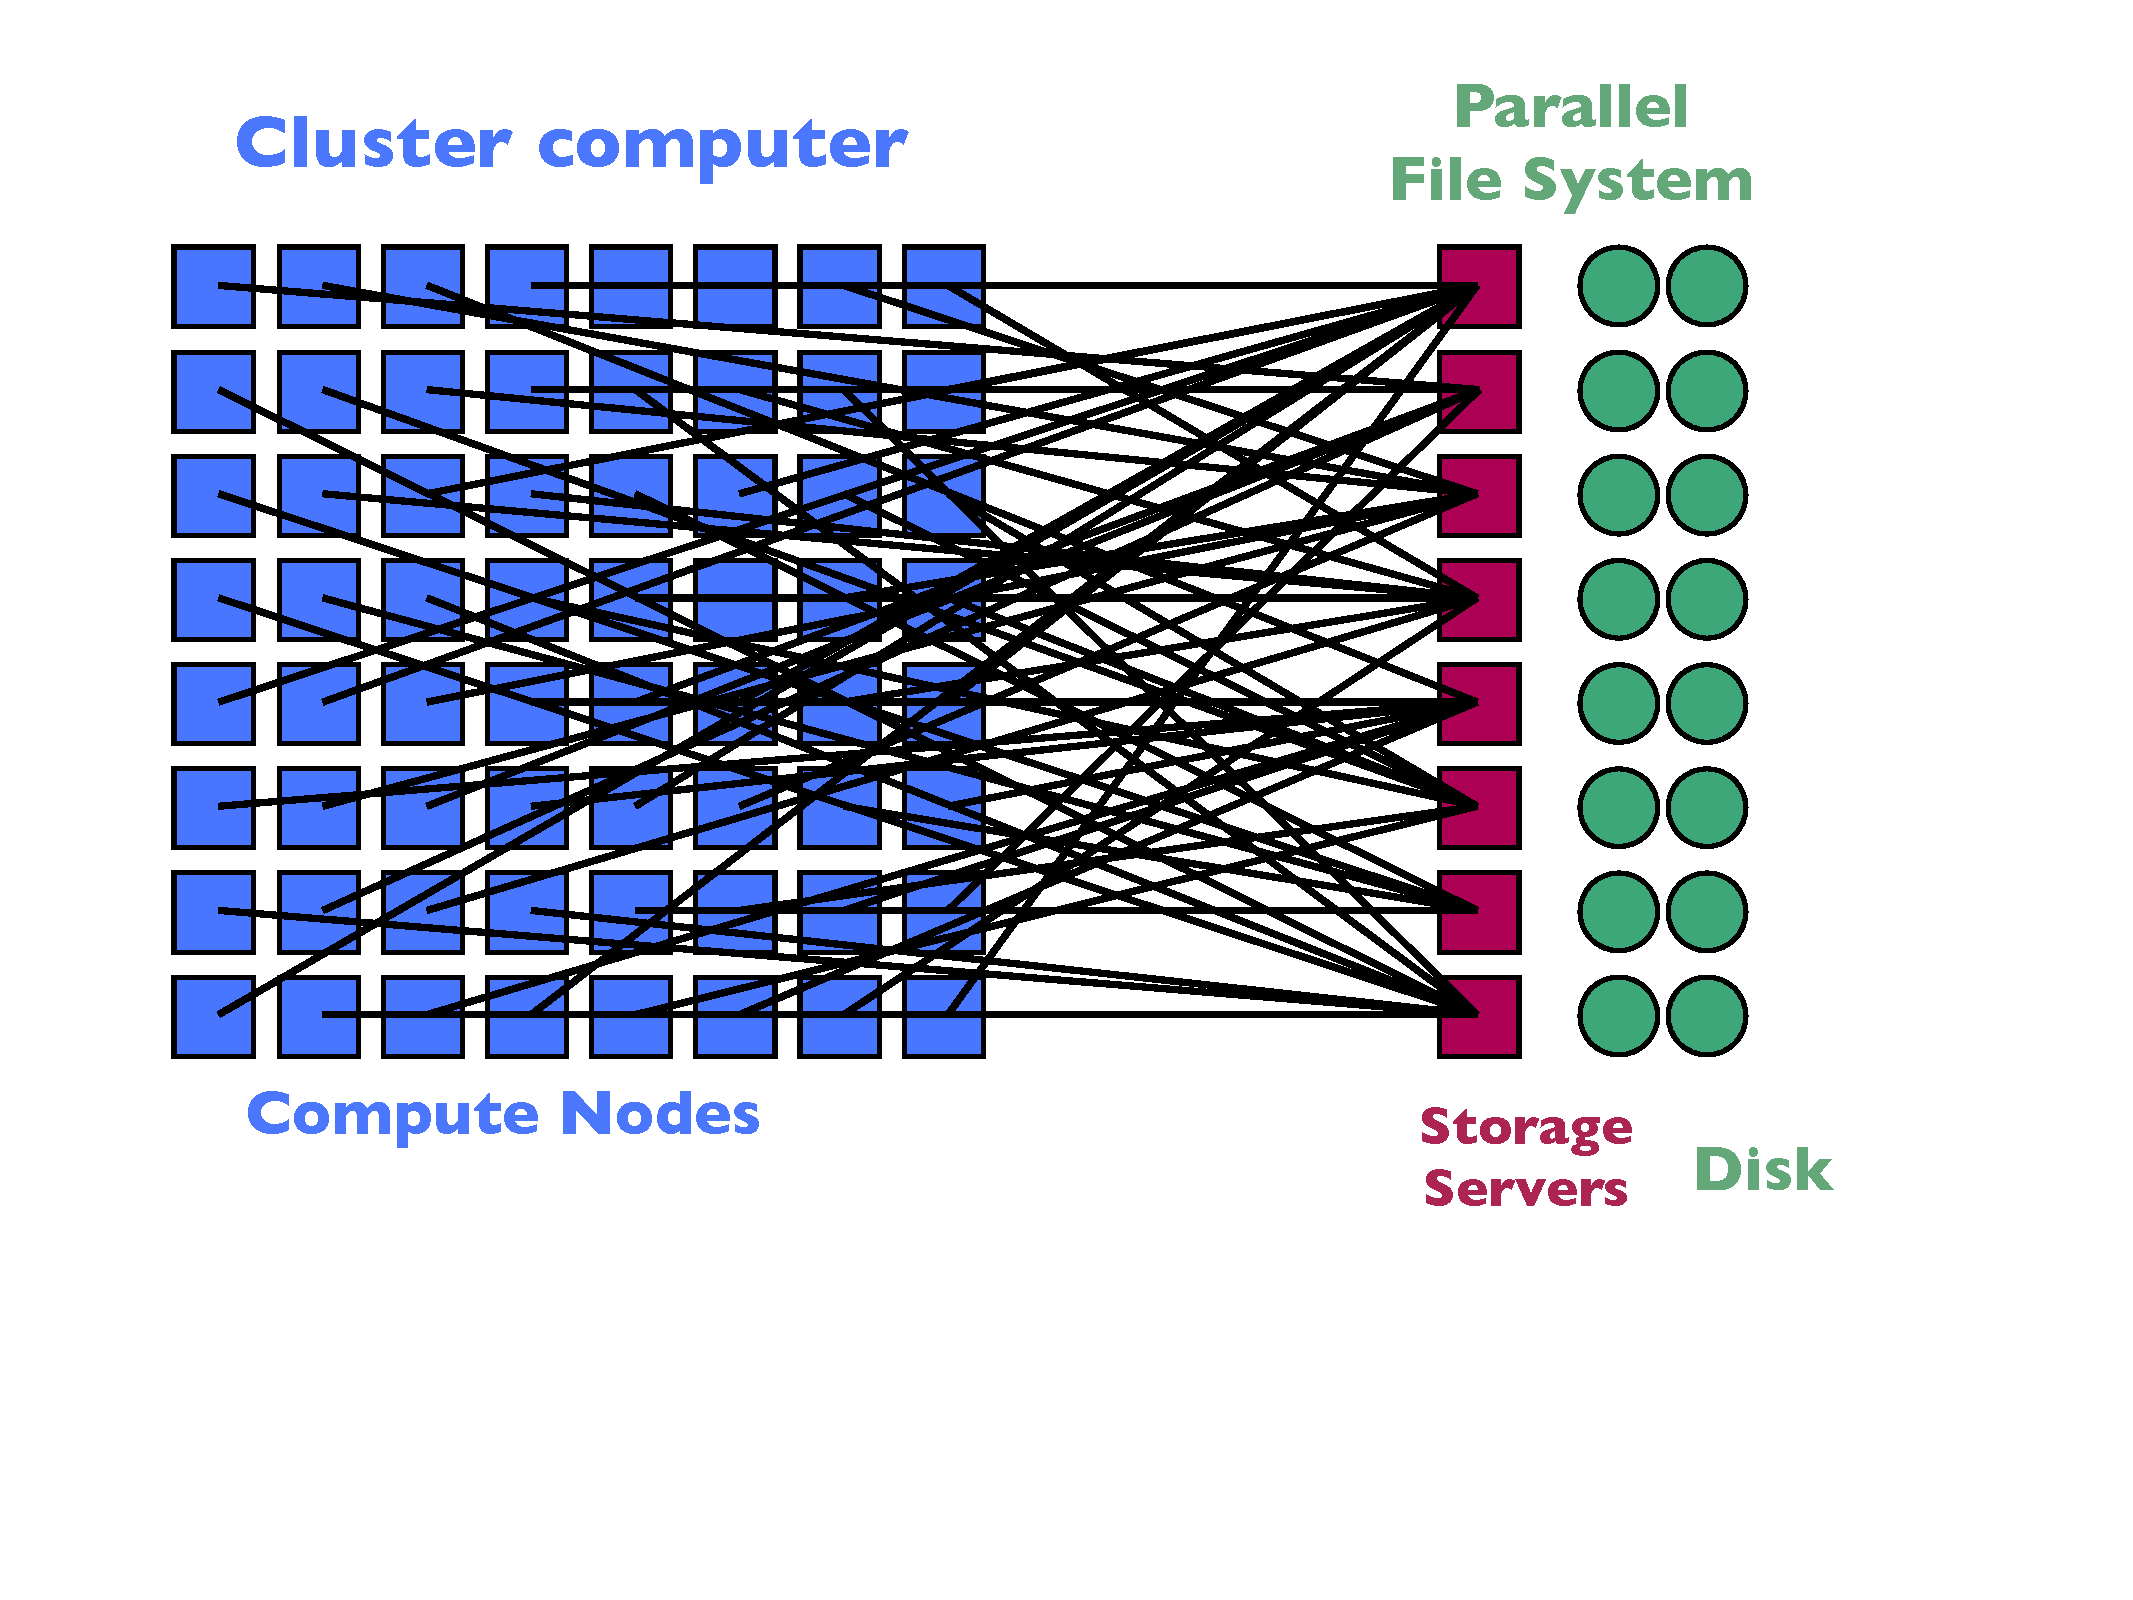
\includegraphics[trim=0 120 30 40,clip,width=1\textwidth]{../common/pics/hardware/ParallelHardware18.pdf}
    \end{block}
  \end{minipage}\hspace{1ex}
  \begin{minipage}{0.32\textwidth}
    \begin{block}{Don't do this!}
      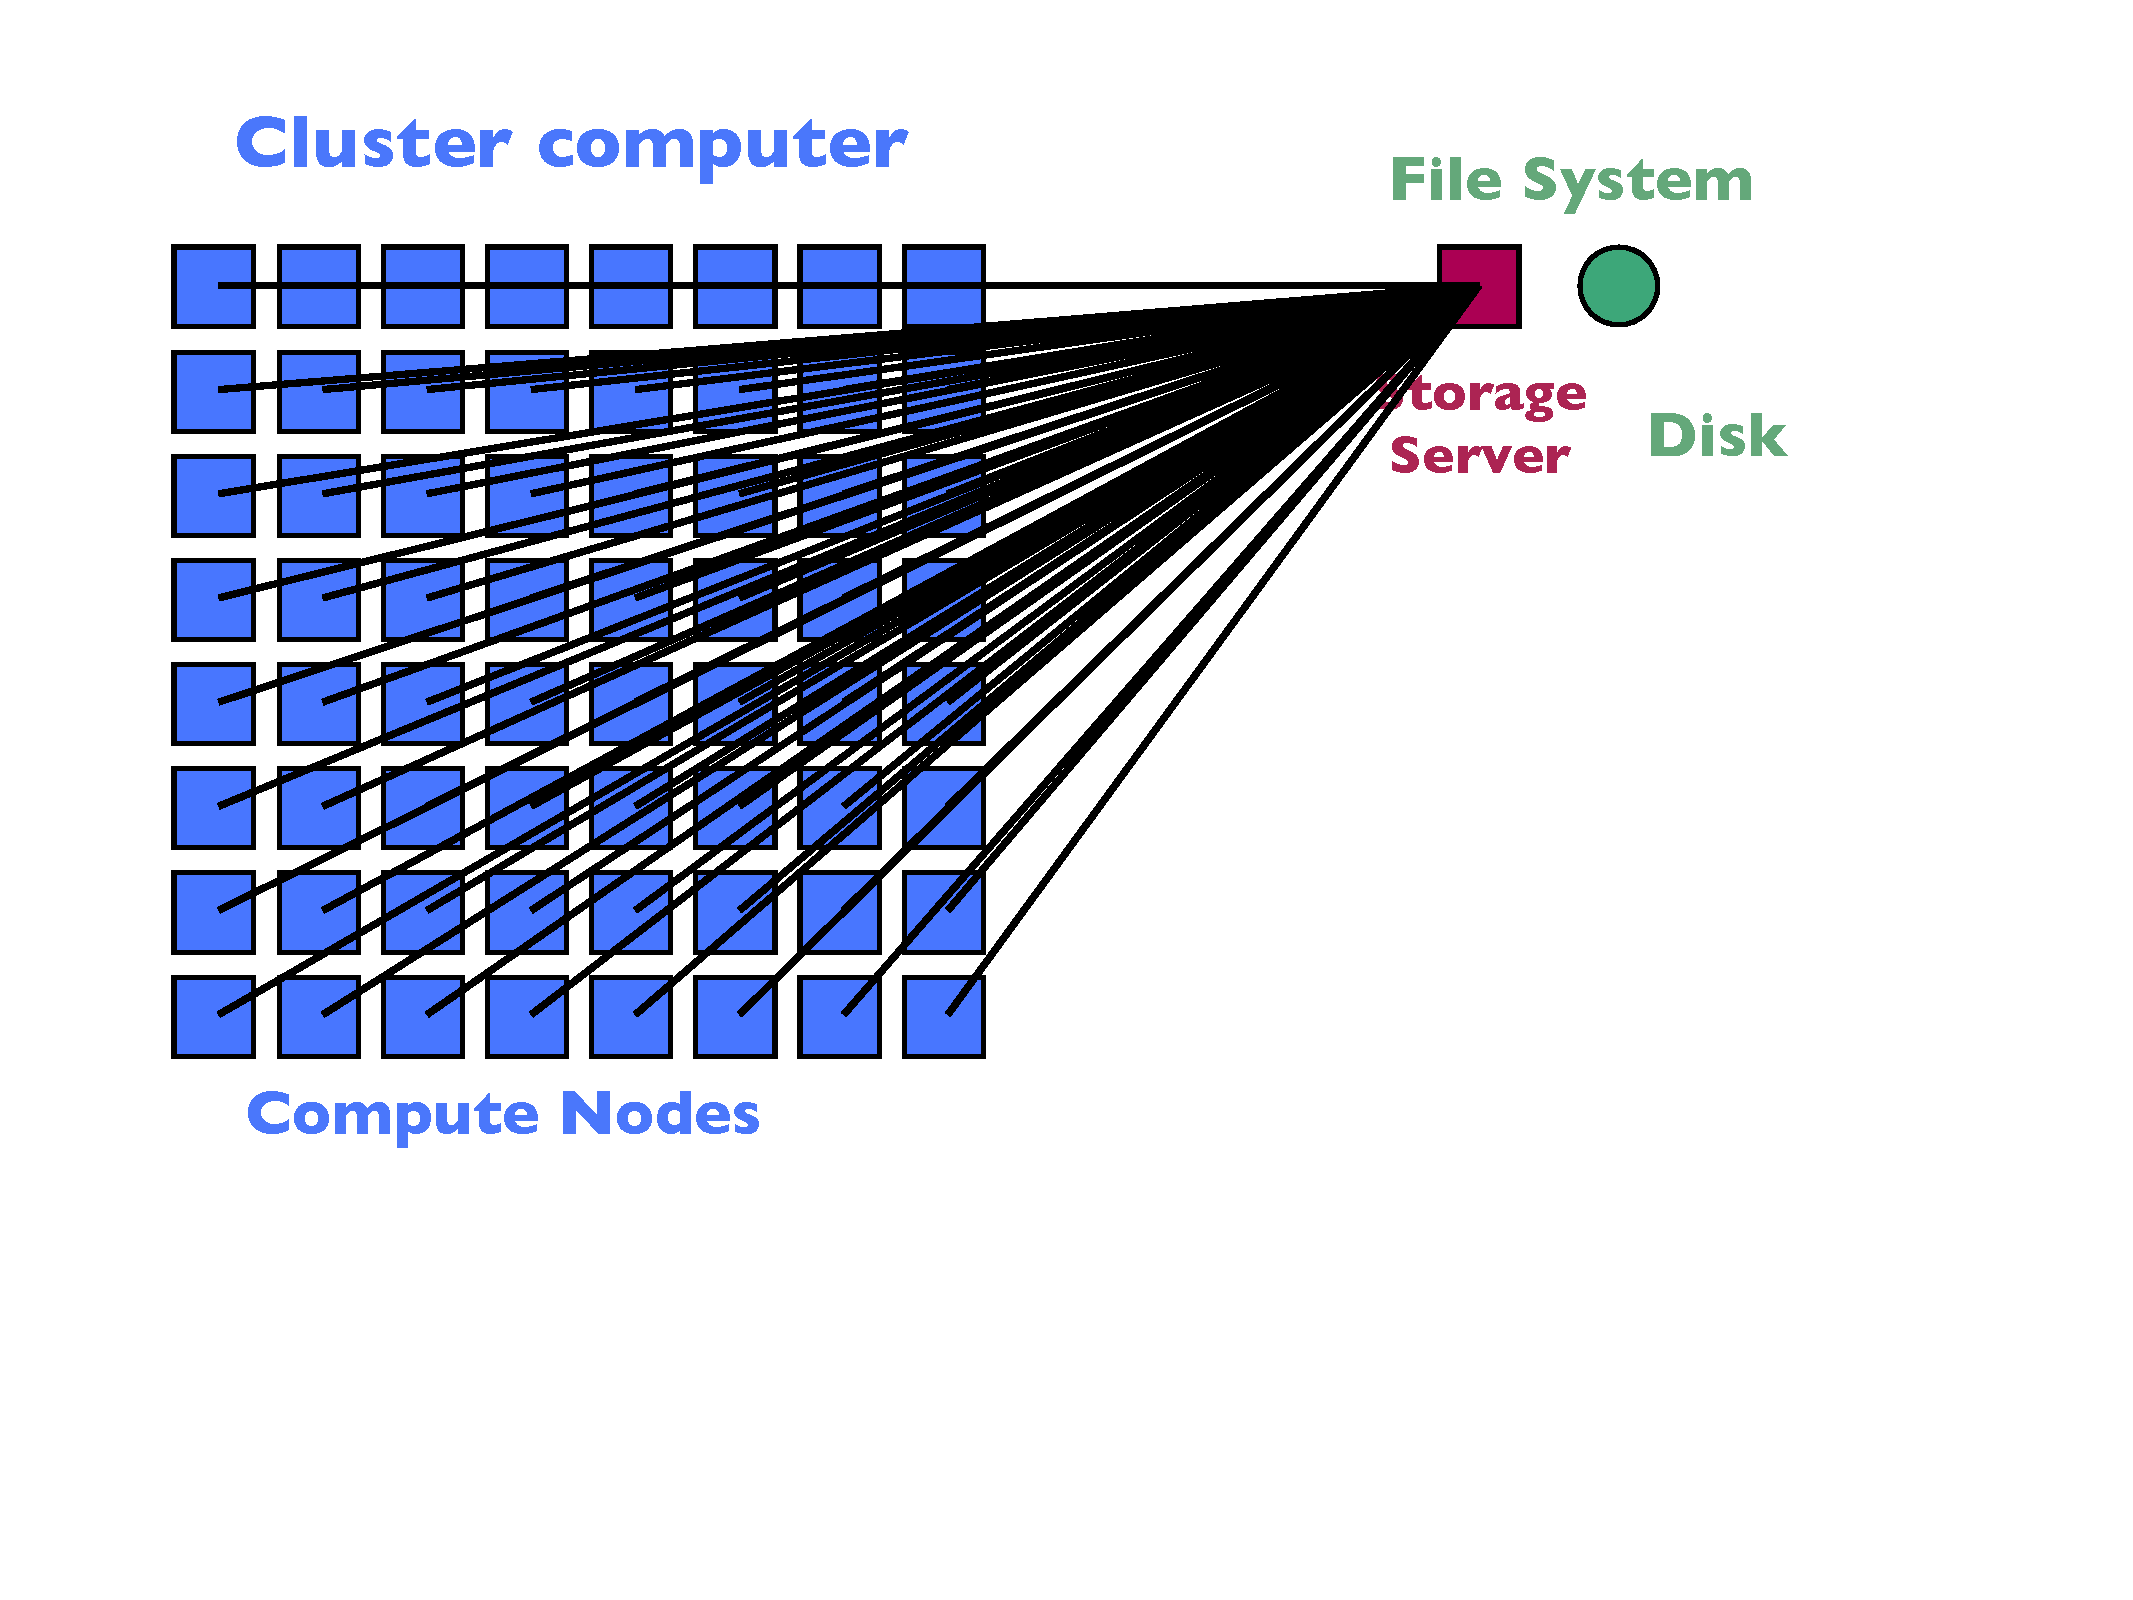
\includegraphics[trim=0 120 30 40,clip,width=1\textwidth]{../common/pics/hardware/ParallelHardware16.pdf}
    \end{block}
  \end{minipage}
\end{frame}


